\sub {

    Just as that round robins are a special case of the more general scheduled formats, multibrackets are a special case of a more general class of formats: \i{networked formats}.

    \begin{definition}{Networked Formats}{}
        A \i{networked format} is a deterministic format in which, after $t_i$ plays $t_j$, the rest of the tournament is identical no matter which team won, except for $t_i$ and $t_j$ are swapped.
    \end{definition}

    Brackets, semibrackets, and multibrackets are clearly networked, though many of their variations are not. Reseeded brackets are not networked, as if a lower-seeded team upsets a higher-seeded team, they will have a tougher road than that higher-seeded team would have. Cohort randomized brackets aren't networked, as there is randomization in the beginning. And perfect double-elimination tournaments like $\D_4$ aren't networked: in the consolidation phase, if the winner of the winners' bracket defeats the winner of the losers bracket, the tournament is over, but if winner of the losers' bracket wins another game is played.

    But the networking property is still a powerful and general frame to view formats with, primarily because we can understand networked formats using \i{network diagrams}. A network diagram contains one horizontal line for each team competing, and vertical lines for each game to played. When two teams play, the winner is moved to the higher horizontal line between the two teams, and the loser is moved to the lower one. Teams are ranked by which horizontal line they end up on.

    % what about formats that do weird rankings. (!! think about this !!)

    For example, recall the 2023 College Football Playoff. Figure \ref{fig:playoff_bracket} displays the format as a bracket, while Figure \ref{fig:playoff_network} displays it as a network diagram.

    \fig{0.82}{playoff_bracket}{The 2023 College Football Playoff Bracket}

    \begin{figg}{The 2023 College Football Playoff Network Diagram}{playoff_network}
        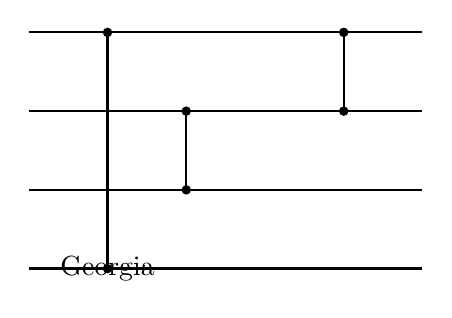
\begin{tikzpicture}
            \foreach \a in {1,...,4}
              \draw[thick] (0,\a) -- ++(5,0);
            \foreach \x in {{1,1},{1,4},{2,2},{2,3},{4,3},{4,4}}
              \filldraw (\x) circle (1.5pt);

            \draw[thick] (1,1) -- (1,4);
            \draw[thick] (2,2) -- (2,3);
            \draw[thick] (4,3) -- (4,4);

            \node[] at (1,1) {Georgia};
            \end{tikzpicture}
    \end{figg}




    % networked representation

    %Recursive Swiss (basically divide into two pools, run this, etc.)

    %Theorem about max games played (vs round robin theorem)

    % cite the art of computing






           % A \i{networked format} is a fixed format in which each game is determined ahead of time to be played between two of
        % \begin{itemize}
        %     \item A specific team,
        %     \item The winner of an earlier game, or
        %     \item The loser of an earlier game,
        % \end{itemize}
        % such that each team, the winner of each game, and the loser of each game are assigned to a game exactly once.




       % A \i{networked format} is a fixed format in which each game is determined ahead of time to be played between two of
        % \begin{itemize}
        %     \item A specific team,
        %     \item The winner of an earlier game, or
        %     \item The loser of an earlier game,
        % \end{itemize}
        % such that each team, the winner of each game, and the loser of each game are assigned to a game exactly once.



        
    % Brackets are networked: each game is indeed between two specific teams, a team and the winner of a previous game, or two winners of previous games; and each team as well as each game-winner is assigned to exactly one game. Multibrackets are similarly networked.

    % In some sense scheduled formats and networked formats are opposites. In one, how a team preforms over course of the format doesn't affect their schedule, and in other, in and other, if two team play, the winner and loser will go to particular next games no matter which is which. However, they are not a disjoint union of the space of scheduled formats.

}